\documentclass[twocolumn]{article}
\usepackage{iasted2}
\usepackage{times}
\usepackage[dvips]{graphicx}

\begin{document}

\title{A SPECKLE REDUCTION ALGORITHM USING THE {\em \`A TROUS} WAVELET TRANSFORM} 
\author{STEWART I. FRASER \\
	Department of Engineering \\
	University of Aberdeen \\  
	Aberdeen, AB24 3UE, UK \\ 
	email: s.i.fraser@abdn.ac.uk \\
	\and
	ALASTAIR R. ALLEN \\
	Department of Engineering \\
	University of Aberdeen \\
        Aberdeen, AB24 3UE, UK \\
        email: a.allen@abdn.ac.uk 
}

\addtolength{\parskip}{0.4cm}

\maketitle
\thispagestyle{empty}

%--------------------------------------------------------------------------------------------------%
\noindent
{\bf\normalsize ABSTRACT}\newline {
Speckle corrupted images are transformed by the shift invariant \emph{\`a trous} (with holes) wavelet transform.
Each wavelet level is then thresholded individually by iteratively approaching the minimum of the difference
between the estimated noise standard deviation and the removed noise standard deviation.
Results of speckle reduction and edge sharpness using this technique, the median filter and the Lee
filter are presented.
An overall quantitative measure for the performance of each filter is ascertained.
Results show that the presented
algorithm performs better overall at reducing speckle whilst preserving edges than the other methods tested.
}
\vspace{2ex}

\noindent
{\bf\normalsize KEY WORDS}\newline {
Image De-noising, Wavelet, Speckle, Filter Evaluation.
}

%--------------------------------------------------------------------------------------------------%
\section{Introduction}
Speckle is caused by the interference of coherent light or waves
which have been scattered from an irregular surface thus giving a granular appearance
to the constructed image. 
Laser holography and
ultrasonic imaging are two techniques susceptive to speckle degradation.  
Since speckle may obscure detail information within an image, 
it can be regarded as noise. This speckle ``noise'' has been identified as multiplicative
in nature, hence causing greater degradation within bright areas of an image than 
in dark areas.
\par Two traditional filters used to de-speckle images are the median filter and the Lee filter \cite{lee80}.
More recently, filters based upon thresholding coefficients of the wavelet transformed image have been 
proposed. For example, 
a soft-thresholding method for optimally recovering 
functions from data with additive Gaussian noise is described in \cite{donoho95}.
The soft-thresholded wavelet coefficients, $\hat{w}$, are obtained from the nonlinear function:
$\hat{w}= {\rm sgn}(w)(|w|-t)_{+}$, where $w$ are the initial wavelet 
coefficients and $t$ is a threshold value.
This threshold value is calculated via: $t=\gamma\sigma\sqrt{2{\rm log}(n)/(n)}$, where $n$ is the number of
data points, $\sigma$ the noise level and $\gamma$ a constant.
\par Variations of this method are used to de-speckle SAR images in \cite{guo94} and ultrasound images 
in \cite{cena96}. In both cases, the logarithmic transform
of the speckle corrupted image is taken to approximate the speckle as Gaussian additive noise
before transforming the image into the wavelet domain.
In \cite{guo94}, both soft-thresholding and hard-thresholding (see Section 3) 
are studied. Hard-thresholding is 
reported to be superior over soft-thresholding for feature preservation, yet inferior to soft-thresholding 
in its ability to reduce speckle.
As an alternative to the optimal soft-thresholding scheme proposed in \cite{donoho95},
an iterative algorithm is described by one of the authors \cite{yu96} to compute an optimal 
hard-thresholding value using a decimated, orthogonal wavelet transform.
Using such a transform results in the noise terms between wavelet levels   
being uncorrelated \cite{lang96} and hence a single threshold value can be applied globally to all the wavelet 
coefficients.
\par Nevertheless, a disadvantage of using a decimated, orthogonal 
wavelet transform as part of a de-noising
algorithm is that the noise reduced image may suffer extensively from visual artifacts such as pseudo-Gibbs phenomena. 
Such phenomena can be attributed to the lack of shift-invariance of the wavelet basis \cite{coifman95}. 
In order to combat this problem, an undecimated, shift invariant, nonorthogonal
wavelet transform can be used. One such
wavelet transform is based upon the \emph{algorithme \`a trous} \cite{stark95, holdschneider89}. 
Using this wavelet transform 
to perform de-noising can significantly reduce the amount of visual artifacts introduced into the noise reduced 
image. 
\par However, applying the wavelet \emph{\`a trous} to a speckle corrupted image will result in the 
noise terms between wavelet levels being correlated \cite{lang96},
thus a different threshold value needs to be calculated for each individual wavelet level.
This paper aims to modify the algorithm proposed in \cite{yu96} which operates in the 
decimated, orthogonal wavelet
domain so that it may be used within an undecimated, 
nonorthogonal wavelet domain. Such a 
modification will result in noise reduced images which are less affected by visual artifacts.  

%--------------------------------------------------------------------------------------------------%
\section{The {\em \`A Trous} Wavelet Transform}
%%%%%%%%%%%%%%%%%%%%%%%%%%%%%%%%%%%%%%%%%%%%%
\subsection{Computing the {\em \`A Trous} Wavelet Transform}
The following explaination is an overview from \cite{stark95, stark98} and describes how the \emph{\`a trous} wavelet
transform can be implemented. 

Using a $B_{3}$-spline scaling function upon the sampled data \{$c_{0}(k)$\},
the smoothed data \{$c_{j}(k)$\} at resolution $j$ and 
position $k$ can be found via:
\begin{displaymath}
	c_{j+1}(k) =	\frac{1}{16}c_{j}(k-2^{j+1})+\frac{1}{4}c_{j}(k-2^{j})+
			\frac{3}{8}c_{j}(k)+ \\
\end{displaymath}
\begin{equation}
			\frac{1}{4}c_{j}(k+2^{j})+\frac{1}{16}c_{j}(k+2^{j+1})
\end{equation}

The signal difference \{$w_{j}(k)$\} between two consecutive resolutions is:
\begin{equation}
	w_{j}(k) = c_{j-1}(k) - c_{j}(k)
\end{equation} 
A series expansion of the original signal, \{$c_{0}(k)$\}, is given by adding all the differences \{$w_{j}(k)$\} 
to the final smoothed array \{$c_{p}(k)$\}:
\begin{equation}
	c_{0}(k) = c_{p}(k) + \sum_{j=1}^{p} w_{j}(k)
\end{equation}

This equation provides a reconstruction formula for the original signal.
At each scale $j$, a set $w_{j}$ is obtained which is called a wavelet level. This has the same
number of pixels as the signal, \emph{i.e.} decimation is not carried out.

In order to extend this algorithm to the two dimensional case, seperability can be assumed for 
the scaling function, \emph{i.e.} a row by row convolution followed by a column by column convolution.

%%%%%%%%%%%%%%%%%%%%%%%%%%%%%%%%%%%%%%%%%%%%%

\subsection{Noise Standard Deviation at each Wavelet Level}
\label{sec:simNoiseImage}

Because the noise terms in the \emph{\`a trous} wavelet transform will be correlated, 
each wavelet level will have a different measure of noise.
A method for obtaining $\sigma_{j}$, the standard deviation of the noise at wavelet level $j$, is
described by \cite{stark95}. This requires $\sigma_{I}$, the standard deviation of the noise within the 
original non-transformed image, along with a study of the noise within the wavelet domain.

In order to study the noise within the wavelet domain, an image containing additive Gaussian noise 
with a standard deviation 
equal to one is simulated. Then the \emph{\`a trous} wavelet transform of this simulated noise 
image is taken and the standard deviation $\sigma_{j}^{s}$ at each wavelet level is computed.
Due to the properties of the wavelet transform, we have: 
\begin{equation}
	\sigma_{j}=\sigma_{I}\sigma_{j}^{s}
	\label{eq:sigmaJ}
\end{equation}

Thus, taking the \emph{\`a trous} wavelet transform of an image,
the standard deviation of the noise at wavelet level $j$ is equal to the standard deviation of the
noise within the original non-transformed image multiplied by the standard deviation of the noise at level $j$
of the wavelet transform.   


%--------------------------------------------------------------------------------------------------%
\section{Thresholding the Wavelet Coefficients}
The algorithm in \cite{yu96} iteratively minimises the difference between the estimated noise standard
deviation and the removed noise standard deviation in order to find an optimal threshold value.
A hard-thresholding scheme is employed to obtain a removed noise component which in turn is used to calculate 
an optimal threshold value which is then applied globally to all wavelet levels. 

In this paper, both soft-thresholding and hard-thresholding are employed to obtain a removed noise component
for each individual wavelet level. These removed noise components are then used to find optimal threshold values for 
each specific wavelet level.

%%%%%%%%%%%%%%%%%%%%%%%%%%%%%%%%%%%%%%%%%%%%%
%\subsection{Hard-Thresholding}
Hard-thresholding implements a \emph{keep or kill} policy, either accepting or rejecting a given wavelet coefficient.
It is expressed by:
\begin{equation}
        \hat{w}_{j} = \left\{ \begin{array}{r@{\quad:\quad}l} w_{j} & \quad\mbox{if}\quad |w_{j}| > t_{j} \\
        0 & \quad\mbox{otherwise}\quad \end{array} \right.
        \label{eq:wHat}
\end{equation}
where, at wavelet level $j$, $w_{j}$ are the wavelet coefficients, $t_{j}$ is the threshold value and
$\hat{w_{j}}$ are the noise reduced coefficients.

%%%%%%%%%%%%%%%%%%%%%%%%%%%%%%%%%%%%%%%%%%%%%
%\subsection{Soft-Thresholding}
Soft-thresholding rejects some wavelet coefficients and shrinks all others towards zero. It is expressed by:
\begin{equation}
        \hat{w}_{j} = \left\{ \begin{array}{r@{\quad:\quad}l} 
	{\rm sgn}(w_{j})(|w_{j}|-t_{j}) & \quad\mbox{if}\quad |w_{j}| > t_{j} \\
        0 & \quad\mbox{if}\quad\mbox{otherwise} \\ 
	\end{array} \right.
        \label{eq:softWHat}
\end{equation}
%where, at wavelet level $j$, $w_{j}$ are the wavelet coefficients, $t_{j}$ is the threshold value
%and $\hat{w}_{j}$ are the noise reduced coefficients.

%%%%%%%%%%%%%%%%%%%%%%%%%%%%%%%%%%%%%%%%%%%%%
%\subsection{Removed Noise Component}
Hard-thresholding (\ref{eq:wHat}) or soft-thresholding (\ref{eq:softWHat}) is applied to a wavelet 
level in order to remove noise. 
Hence, this removed noise component can be given by: 
\begin{equation}
	\check{w}_{j} = w_{j} - \hat{w}_{j}
        \label{eq:wCheck}
\end{equation}
%where, at wavelet level $j$, $w_{j}$ are the wavelet coefficients and 
%$\hat{w}_{j}$ are the noise reduced coefficients. 
Either (\ref{eq:wHat}) or (\ref{eq:softWHat}) can be used to calculate $\hat{w}_{j}$.

%%%%%%%%%%%%%%%%%%%%%%%%%%%%%%%%%%%%%%%%%%%%%
%\subsection{Optimising the Threshold Value}
For a given threshold value $t_{j}$ at wavelet level $j$, a removed noise component can be obtained. A
measure of this reduced noise component is used to adjust the threshold $t_{j}$ to obtain an optimal 
threshold value for each wavelet level. To do this, a performance function is set:
\begin{equation}
        f = \min \{ \sigma_{j} - \sigma_{j}^{r} \}
        \label{eq:performFunction}
\end{equation}
where $\sigma_{j}$ is the estimated standard deviation of the noise for wavelet level $j$
and $\sigma_{j}^{r}$ is the standard deviation of the removed noise obtained from wavelet level $j$.
The goal is to find the optimal $t_{j}$ for each wavelet level so that (\ref{eq:performFunction})
approaches a minimum.

%--------------------------------------------------------------------------------------------------%
\section{The Algorithm}

The iterative algorithm used to find threshold values for each level of a speckle corrupted image
transformed by the \emph{\`a trous} wavelet transform is as follows:
\newcounter{step}
\begin{list}{\arabic{step}.}{ \usecounter{step}
\setlength{\labelwidth} {0.5cm} \rm }
	\item Logarithmically transform the speckle corrupted image thus
	approximating the speckle as Gaussian additive noise.
		
	\item Compute $p$ levels of the \emph{\`a trous} wavelet transform for the logarithmically
	transformed image. 

	\item Estimate $\sigma_{I}$, the level of noise within the image, by calculating the standard deviation 
	of the coefficients within the
	first level of the wavelet transform. These coefficients are due mainly to the noise.
	
	\item Simulate an image containing additive Gaussian noise with a standard deviation equal to one
	(as described in Section \ref{sec:simNoiseImage})
	and compute $p$ levels of the \emph{\`a trous} wavelet transform for it. 
	For each wavelet level $j$ of this simulated noise image, calculate the standard deviation $\sigma_{j}^{s}$.

	\item At each wavelet level $j$ of the logarithmically transformed speckle corrupted image, 
	estimate the standard deviation of the noise: $\sigma_{j}=\sigma_{I}\sigma_{j}^{s}$. 
	
	\item Set $j=0$.
	
	\item $j=j+1$.
	\label{step:incrementJ}

	\item Set initial threshold value for wavelet level $j$; $t_{j} = t_{0}$. 

	\item 
	\begin{tabbing}
	If \= $j = 1$ \\
	\>Using soft-thresholding, obtain the removed noise \\ 
	\>component $\check{w}_{j}$ from (\ref{eq:wCheck}). \\

	Else \\
	\>Using hard-thresholding, obtain the removed noise \\
	\>component $\check{w}_{j}$ from (\ref{eq:wCheck}). 
	\end{tabbing}
	\label{step:sh_if1}

	\item Calculate $\sigma_{j}^{r}$, the standard deviation of the removed noise component.

	\item Compute $\Delta = \sigma_{j} - \sigma_{j}^{r}$.
	
	\item 
	\begin{tabbing}
	If \= $\Delta$ $\leq K$ and $j = 1$ \\
	\>Using soft-thresholding, obtain the de-noised \\
	\>wavelet coefficients $\hat{w}_{j}$ from (\ref{eq:softWHat}), then go to \\ 
	\>step \ref{step:jLeqP}. \\
	Else if $\Delta \leq K$ \\
	\>Using hard-thresholding, obtain the de-noised \\
	\>wavelet coefficients $\hat{w}_{j}$ from (\ref{eq:wHat}), then go to \\
	\>step \ref{step:jLeqP}. \\
	\end{tabbing}
	\label{step:sh_if2}

	\item Renew threshold $t_{j} = t_{j} + k\Delta$. Go to step \ref{step:sh_if1}.

	\item
	\begin{tabbing}
	If \= $j < p$ \\
	\> Go to step \ref{step:incrementJ}. \\
	\end{tabbing}
	\label{step:jLeqP}

	\item Construct the thresholded image $\tilde{c}_{0}$ via
	\begin{equation}
		\tilde{c}_{0} = c_{p} + \sum_{j=1}^{p} \hat{w}_{j}
	\end{equation}
	where $c_{p}$ is the final smoothed image and
	$\hat{w}_{j}$ are the de-noised wavelet levels.
	
	\item Obtain the de-speckled image by applying the exponential transform (inverse of logarithmic
	transform) upon thresholded image $\tilde{c}_{0}$. 
\end{list}
where $K$ is the tolarence of (\ref{eq:performFunction}) and $k$ is the step size for each threshold 
value $t_{j}$. 

As was suggested in \cite{zong98},
different thresholding schemes can be applied to different wavelet levels. 
Soft-thresholding has the advantage of providing a high level of smoothness while hard-thresholding
preserves features well. Hence, it is prudent to apply a soft-thresholding scheme at fine levels
of the wavelet transform where the noise is most prevalent and a hard-thresholding scheme at coarser levels where the 
noise is not as prevalent. 
The above algorithm implements soft-thresholding upon the finest wavelet level and hard-thresholding upon all other levels
(see algorithm steps \ref{step:sh_if1} and \ref{step:sh_if2}). Such a scheme gave the best results for de-speckling 
the test images in Section \ref{sec:results}

%--------------------------------------------------------------------------------------------------%
\section{Results}
\label{sec:results}

The results of the algorithm described in Section 4 are compared with those of 
the median filter and the Lee filter. 
Slightly modified versions of the comparison criteria  
used in \cite{lee94,yu96} are used here, namely: 
\begin{itemize}
	\item {\bf Speckle strength within homogeneous regions.} \\
	Within a homogeneous region of the image, the standard deviation to mean ratio 
	is used to assess the level of speckle strength.
	Speckle reduction ($SR$) within a homogeneous region is given by:
	\begin{equation}
		SR = 1 - \frac	{\parbox[h]{4.75cm}{\centering \emph{speckle~strength~after~filtering}}}
				{\parbox[h]{4.75cm}{\centering \emph{speckle~strength~before~filtering}}}
	\end{equation}

	\item {\bf Edge sharpness.} \\
	Strips of width three pixels on both sides of an edge are used to determine 
	the edge sharpness. The mean of each strip is calculated and the
	absolute difference is taken as a measure of the edge sharpness.
	Edge sharpness ($ES$) is given by:
	\begin{equation}
		ES = \frac	{\parbox[h]{4.75cm}{\centering \emph{edge~sharpness~after~filtering}}}
				{\parbox[h]{4.75cm}{\centering \emph{edge~sharpness~before~filtering}}}
	\end{equation}
\end{itemize}

Using $7\times7$ windows, $SR$ and $ES$ are both measured three times within separate locations for each de-speckled image.
These results are then averaged, producing an overall speckle reduction ($\overline{SR}$) value and an overall edge 
sharpness value ($\overline{ES}$).
In~\cite{jimenez01}, a global restoration index was introduced which assigned an overall rating to the
performance of a filter. This was achieved by having a noise reduction measurement and a discontinuity preservation 
measurement, both of which were bounded to the range 0-1. 
A modified version of the technique described in~\cite{jimenez01} is incorporated here to quantify the overall performance of a filter. 
Using $\overline{SR}$ as the noise reduction measurement and $\overline{ES}$ as the discontinuity preservation measurement, 
the filter performance ($FP$) is calculated via: 
\begin{equation}
\label{eq:fp}
	FP= \sqrt { \overline{SR} \cdot \overline{ES}}
\end{equation}
Thus, all $FP$ values are bounded to the range 0-1, where values near 1 indicate high quality restoration 
and values close to zero represent poor quality restoration.

The median filter was implemented each time using a $7\times7$ window.
The parameters for the wavelet filter and the Lee filter were chosen to give
de-speckled images with identical PSNR (peak signal to noise ratio) values.
Four levels of the wavelet \emph{\`a trous} were computed.
All three filters were applied to four common test images, each of which had been corrupted with speckle. 
For each test image, Table 1 shows the PSNR values prior to and after filtering.

\begin{table}[ht]
\begin{center}
\begin{footnotesize}
\begin{tabular}{|l|c|c|c|c|} \hline
 		& Lena		& Peppers	& F16 		& Goldhill 	\\ \hline
original	& 24.16 dB	& 22.90 dB	& 19.94 dB	& 23.59 dB	\\ \hline
median		& 25.03 dB	& 24.35 dB	& 21.91 dB	& 23.63 dB	\\ \hline
Lee		& 29.32 dB	& 28.22 dB	& 25.92 dB	& 26.75 dB	\\ \hline
wavelet		& 29.32 dB	& 28.22 dB	& 25.92 dB	& 26.75 dB	\\ \hline
\end{tabular}
\end{footnotesize}
\end{center}
\begin{minipage}[h]{8.3cm}
	{\begin{center} Table 1. PSNR values prior to and after filtering for each of the four test images. \end{center}}
\end{minipage}
\end{table}


In Table 2, the quantitative results for the performance of each filter are displayed. In this table,
the bold values represent the best performing filter for a particular comparison criterion within each test image.
It can be seen that the highest level of speckle reduction is obtained using the wavelet filter, followed
by the median filter with the Lee filter performing the poorest. 
The Lee filter marginally surpasses the wavelet filter at maintaining edge sharpness whereas the median filter performs 
the worst.
Overall, the wavelet filter is seen to perform the best, giving excellent speckle reduction combined with 
a high degree of edge sharpness. Figures 1(a), (b), (c) and (d)
show the original Lena image corrupted with speckle and the results of applying the tested filters upon it.

%------------------------------------------------------------------------------------------------%
\begin{table}[ht]
\begin{center}
\begin{footnotesize}
\begin{tabular}{|l|c|c|c|c|} \hline
				& Lena 		& Peppers 	& F16 		& Goldhill 	\\ \hline \hline
Speckle reduction median	& 0.75		& 0.71		& 0.78		& 0.78		\\ \hline
Speckle reduction Lee		& 0.68		& 0.64		& 0.76		& 0.71		\\ \hline
Speckle reduction wavelet	& {\bf 0.78}	& {\bf 0.75}	& {\bf 0.92}	& {\bf 0.84}	\\ \hline \hline
Edge sharpness median		& 0.70		& 0.83		& 0.79		& 0.83		\\ \hline
Edge sharpness Lee		& {\bf 0.92}	& {\bf 0.95}	& {\bf 0.96}	& {\bf 0.93}	\\ \hline
Edge sharpness wavelet		& 0.90		& 0.92		& 0.90		& 0.92		\\ \hline \hline
Filter performance median	& 0.72		& 0.77		& 0.78		& 0.80		\\ \hline
Filter performance Lee		& 0.79		& 0.78		& 0.85		& 0.81		\\ \hline
Filter performance wavelet	& {\bf 0.84}	& {\bf 0.83}	& {\bf 0.91}	& {\bf 0.88}	\\ \hline
\end{tabular}
\end{footnotesize}
\end{center}
\begin{minipage}[h]{8.3cm}
	{\begin{center} Table 2. Quantitative results (bounded to range 0-1). \end{center}} 
\end{minipage}
\end{table}

%------------------------------------------------------------------------------------------------%
\section{Conclusion}
A novel iterative filtering technique operating in the shift invariant \emph{\`a trous} wavelet
domain has been presented. This speckle reduction algorithm was compared to both the median and
Lee filters. For speckle reduced images of equal PSNR, the presented filtering technique was seen 
to give marginally less edge preservation but a much greater degree of speckle reduction 
when compared to the Lee filter.
This ability of the Lee filter to preserve edges is tempered by the fact that its capacity to remove
speckle from edge regions within the image is extremely poor.
The median filter was seen to give good speckle reduction, but this was achieved at 
the expense of edge preservation.

Future work will focus upon testing the algorithm with various diagnostic ultrasound images. 
Such images have the added problem that 
the speckle ``texture'' conveys information to the expert viewer, hence making it difficult
to find a suitable balance between de-speckling and texture preservation. 

%--------------------------------------------------------------------------------------------------%
\begin{thebibliography}{00}
	\bibitem{lee80}J. S. Lee, Digital image enhancement and noise filtering by use of local
	statistics, \emph{IEEE Transactions PAMI}, Vol. PAMI-2, No. 2, 1980, 165-168.

	\bibitem{donoho95}D. L. Donoho, De-noising by soft-thresholding,
	\emph{IEEE Transactions on Information Theory}, Vol. 41, No. 3, 1995, 613-627.

	\bibitem{guo94}H. Guo, J. E. Odegard, M. Lang and R. A. Gopinath, Wavelet based speckle reduction
	with application to SAR based ATD/R, \emph{IEEE International Conference on Image Processing},
        Austin, USA, 1994, 75-79. 

	\bibitem{cena96}B. Cena and N. Spadaccini, Wavelet shrinkage of ultrasound data,
	\emph{Summer School on Wavelets: Papers}, Zakopane, Poland, 1996, 11-18.
	
	\bibitem{yu96}R. Yu, A. R. Allen and J. Watson, An optimal wavelet thresholding method
	for speckle noise reduction, \emph{Summer School on Wavelets: Papers},
	Zakopane, Poland, 1996, 77-81.

	\bibitem{lang96}M. Lang, H. Guo, J. E. Odegard, C. S. Burrus and R. O. Wells, Jr,
	Noise reduction using an undecimated discrete wavelet transform,
	\emph{IEEE Signal Processing Letters}, Vol. 3, No. 1, 1996, 10-12.

	\bibitem{coifman95}R. R. Coifman and D. L. Donoho, Translation-invariant de-noising,
	in A. Antoniadis and G. Oppenheim (Eds.) \emph{Wavelets and Statistics} (New York:
	Springer-Verlag, 1995), 125-150.
	%(www-stat.stanford.edu/~donoho/Reports/index.html)

	\bibitem{stark95}J. L. Starck, F. Murtagh and A. Bijaoui, Multiresolutional support 
	applied to image filtering and restoration, \emph{Graphical Models and Image
	Processing}, Vol. 57, 1995, 420-431.

	\bibitem{holdschneider89}M. Holdschneider, R. Kronland-Martinet, J. Morlet, Ph. Tchamitchian, 
	A real-time algorithm for signal analysis with the help of the wavelet transform, 
	in J. M. Combes, A. Grossmann and Ph. Tchamitchian (Eds.) \emph{Wavelets} (Berlin:
	Springer-Verlag, 1989), 286-297.

	\bibitem{stark98}J. L. Starck, F. Murtagh and A. Bijaoui, \emph{Image Processing and 
	Data Analysis - The Multiscale Approach}, Cambridge University Press, 1998.

	\bibitem{zong98}X. Zong, A. F. Laine and E. A. Geiser, Speckle reduction and contrast enhancement
	of echocardiograms via multiscale nonlinear processing, \emph{IEEE Transactions on Medical Imaging},
	Vol. 17, No. 4, 1998, 532-540.
	
	\bibitem{lee94}J. S. Lee, I. Jurkevich, P. Dewaele, P. Wambacq and A. Oosterlinck,
	Speckle filtering of synthetic aperture radar
	images: a review, \emph{Remote Sensing Reviews}, Vol. 8, 1994, 313-340.

	\bibitem{jimenez01}A. R. Jim\'enez, R. Ceres and J. L. Pons, A new adaptive filter and quality
	evaluation index for image restoration, \emph{The Journal of the Pattern Recognition Society},
	Vol. 34, No. 2, 2001, 457-467.
\end{thebibliography}

\newpage
\clearpage
\onecolumn
\begin{figure}[h]
	\begin{minipage}[h]{8.3cm} {\begin{center} 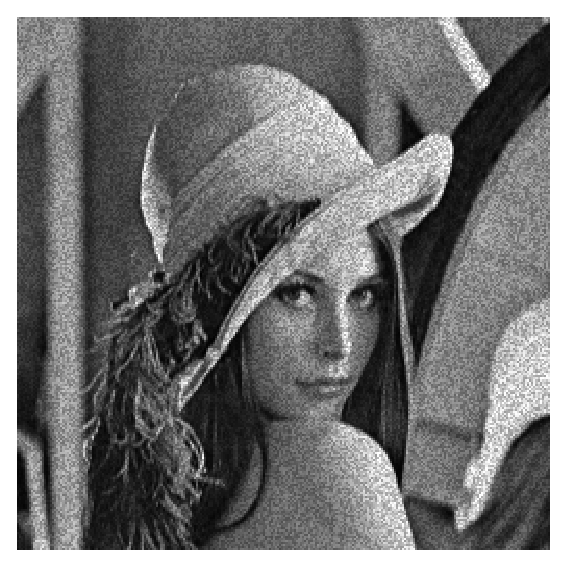
\includegraphics[height=8.05cm,width=8.05cm]{../../pics/lena_noisy.ps} \\(a) \end{center}} \end{minipage}
	\hspace{1.2cm}
	\begin{minipage}[h]{8.3cm} {\begin{center} 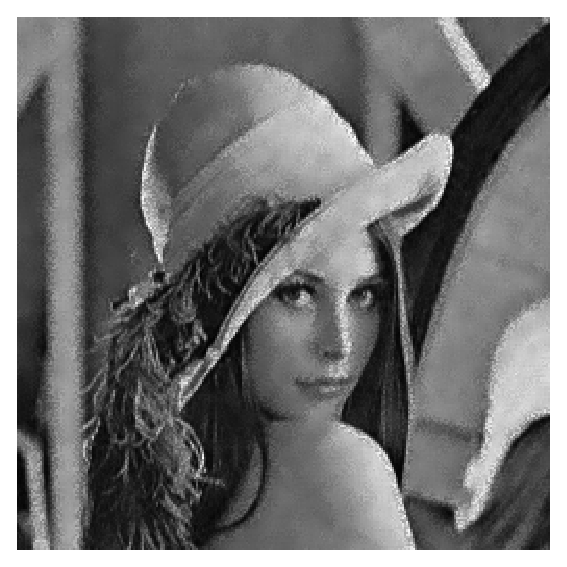
\includegraphics[height=8.05cm,width=8.05cm]{../../pics/lena_lee.ps} \\(c) \end{center}} \end{minipage}
\end{figure}
\begin{figure}[h]
	\begin{minipage}[h]{8.3cm} {\begin{center} 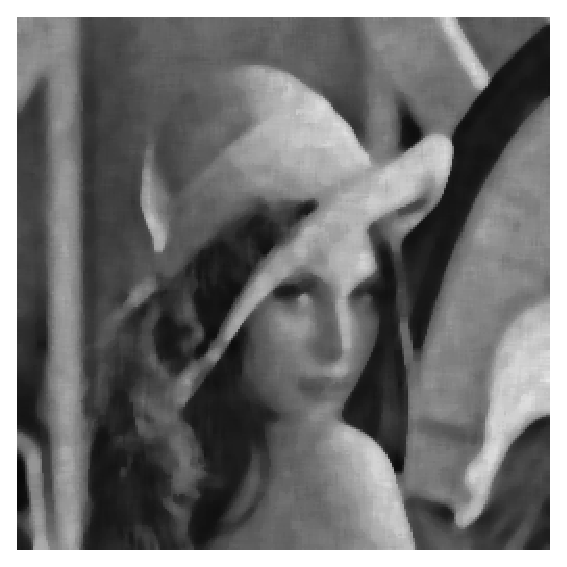
\includegraphics[height=8.05cm,width=8.05cm]{../../pics/lena_med7.ps} \\(b) \end{center}} \end{minipage}
	\hspace{1.2cm}
	\begin{minipage}[h]{8.3cm} {\begin{center} 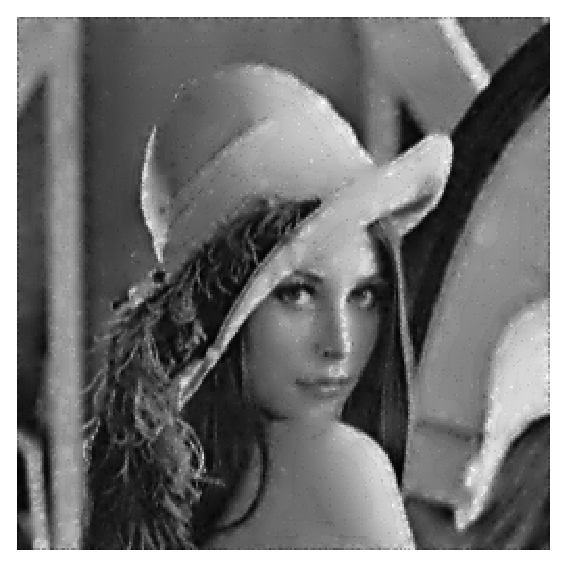
\includegraphics[height=8.05cm,width=8.05cm]{../../pics/lena_yu_1.165n.ps} \\(d) \end{center}} \end{minipage}
\end{figure}
\begin{minipage}[h]{16.6cm}
	{\begin{center} Figure 1. (a) Lena corrupted with speckle. (b) Median filter result. (c) Lee filter result. (d) Wavelet filter result. \end{center}}
\end{minipage}


\end{document}
